\chapter{Installazione}
Per utilizzare l'applicazione web è necessario:
\begin{itemize}
  \item Clonare il repository;
  \item Avviare il server;
  \item Avviare la web app.
\end{itemize}
\section{Clonare il repository}
\begin{itemize}
  \item Scaricare il codice come file .zip direttamente dal repository \textit{login-warrior}:
  \begin{center}
    \url{https://github.com/merlunipd/login-warrior}
  \end{center}
  oppure, avendo \textit{Git} installato in locale, è possibile clonare il repository con il comando:
  \begin{center}
    \textcolor{purple}{\texttt{git clone https://github.com/merlunipd/login-warrior}}
  \end{center}
  \item Localizzare da terminale la cartella in cui è stato estratto/clonato il prodotto:
  \begin{center}
    \textcolor{purple}{\texttt{cd percorso\textbackslash LoginWarrior}}
  \end{center}
\end{itemize}

\section{Avviare il server}
\begin{itemize}
  \item Entrare nella cartella \texttt{login$\_$warrior} con i seguenti comandi:
  \begin{center}
    \textcolor{purple}{\texttt{cd src} \\
    \texttt{cd login$\_$warrior}}
  \end{center}
  \item In caso di primo avvio, per crea la cartella \texttt{node$\_$modules} dove vengono installate tutte le dipendenza necessarie digitare:
  \begin{center}
    \textcolor{purple}{\texttt{npm install}}
  \end{center}
  \item Per listare gli script impostati digitare (\textbf{Opzionale}):
  \begin{center}
    \textcolor{purple}{\texttt{npm run}}
  \end{center}
  \item Per eseguire un server locale che permette l'accesso all'applicazione digitare:
  \begin{center}
    \textcolor{purple}{\texttt{npm run server}}
  \end{center}
\end{itemize}

\section{Avviare la web app}
Dopo aver avviato il server come spiegato nel passo precedente, l'applicazione sarà disponibile aprendo l'indirizzo fornito dal terminale:
\begin{figure}[ht]
	\centering
	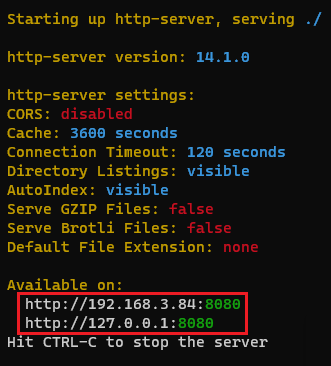
\includegraphics[width=200px]{server.png}
	\caption{Avvio dell'applicazione}
  \end{figure}
